\documentclass{beamer}

\usepackage{fontspec,xunicode,xltxtra}
\usepackage[english]{babel}
\usepackage{microtype}
\usepackage{default}

\usepackage[]{hyperref}
\hypersetup{
	colorlinks=true}
\usetheme{simple}
\usepackage{graphicx}
\usepackage[justification=centering]{caption}
\usepackage{subcaption}
\usepackage{listings}
\usepackage{pstricks}
\setmainfont{Fira Sans}
\setsansfont{Noto Sans}
\setmonofont{Fira Code}
\captionsetup[subfigure]{labelformat=empty}
\captionsetup[figure]{labelformat=empty}
\setbeamertemplate{caption}{\raggedright\insertcaption\par}
\setbeamerfont{frametitle}{size=\LARGE}
\newfontfamily\DejaSans{DejaVu Sans}
\setbeamerfont{title}{family=\texttt,size=\huge}
\usepackage[scale=2]{ccicons}
\newfontfamily\unicodefun[Ligatures=TeX]{Symbola}
\newfontfamily\unicodefun{Droid Sans}


\lstdefinelanguage{JavaScript}{
    keywords={typeof, new, true, false, catch, function, return, null, catch, switch, var, if, in, while, do, else, case, break},
    keywordstyle=\color{blue}\bfseries,
    ndkeywords={class, export, boolean, throw, implements, import, this},
    ndkeywordstyle=\color{darkgray}\bfseries,
    identifierstyle=\color{black},
    sensitive=false,
    comment=[l]{//},
    morecomment=[s]{/*}{*/},
    commentstyle=\color{purple}\ttfamily,
    stringstyle=\color{red}\ttfamily,
    morestring=[b]',
    morestring=[b]"
}

\lstset{
    language=JavaScript,
    extendedchars=true,
    basicstyle=\footnotesize\ttfamily,
    showstringspaces=false,
    showspaces=false,
    numberstyle=\footnotesize,
    numbersep=9pt,
    tabsize=2,
    breaklines=true,
    showtabs=false,
    captionpos=b
}

\title{Graphical Temporal Structured Programming}
\subtitle{}
\date{}
\author{Jean-Michaël Celerier$\mathsf{^{1,2,3}}$~\\ Myriam Desainte-Catherine$\mathsf{^{2,3}}$~\\ Jean-Michel Couturier$\mathsf{^{1}}$}
\institute{1. Blue Yeti --- 2. SCRIME / LaBRI --- 3. PoSET}
\titlegraphic{
    
\includegraphics[width=0.2\textwidth]{images/logobl.png} \vspace{1cm}
    
\includegraphics[width=0.2\textwidth]{images/poset.png} \vspace{1cm}
    
\includegraphics[width=0.5\textwidth]{images/scrime.jpg}}

\usepackage{tikz}

\newsavebox{\codebox}% For storing listings
\begin{document}
    
\maketitle
\begin{frame}
	\tableofcontents
\end{frame}
\section{Introduction}
\subsection{Position}
\begin{frame}
    \frametitle{Position}    
    \Large
    \vspace{5mm}
    
    % TODO diagramme interactivité de la pres 1A
    Authoring \textbf{interactivity} ?
    \vspace{5mm}
    
    \hfill \emph{When A then B : \textbf{programming}}
    \vspace{5mm}
    
    \textbf{Code-first} environments.
    \vspace{5mm}
    
    \hfill \emph{Previous i-score version: \textbf{interaction points}.}
    \vspace{5mm}
    
    \small
    \begin{figure}
        \begin{tikzpicture}
        \draw[thick] (0,0) -- (8,0) 
        node (L0) [at start] {$\bullet$}
        node (L1) [very near start] {}
        node (L2) [midway] {}
        node (L3) [near end] {}
        node (L4) [at end] {$\bullet$}
        
        node [at start, above, yshift=0.2cm] {Logical}
        node [at end, above, yshift=0.2cm] {Temporal}
        
        node (T0) [at start, below, yshift=-0.2cm] {Pure code}
        node (T1) [very near start, below, text width=5cm, yshift=-1cm, text centered] {Max~\\game engines}
        node (T2) [midway, below, text width=5cm, yshift=-0.2cm, text centered] {MaxScore~\\note\textasciitilde}
        node (T3) [near end, below, yshift=-0.4cm] {i-score}
        node (T4) [at end, below, text width=3.5cm, yshift=-1cm, text centered] {Sequencers~\\(Cubase, Final Cut...)}
        ;
        
        \draw[thick] (L0) ++(0,0.2) -- (T0);
        \draw[thick] (L1) ++(0,0.2) -- (T1);
        \draw[thick] (L2) ++(0,0.2) -- (T2);
        \draw[thick] (L3) ++(0,0.2) -- (T3);
        \draw[thick] (L4) ++(0,0.2) -- (T4);
        \end{tikzpicture}
    \end{figure}
\end{frame}

\subsection{Inspiration}
\begin{frame}
    \frametitle{Inspiration}
    \Large
    \begin{columns}
        \begin{column}{0.45\textwidth}
            Polyvalent structure:
            \begin{itemize}
                \item \textbf{Feldman}~\\\textit{Intermission}
                \item \textbf{Cage}~\\\textit{Two}
                \item \textbf{Stockhausen}~\\\textit{Klavierstück XI}
            \end{itemize}
        \end{column}
        \begin{column}{0.45\textwidth}
            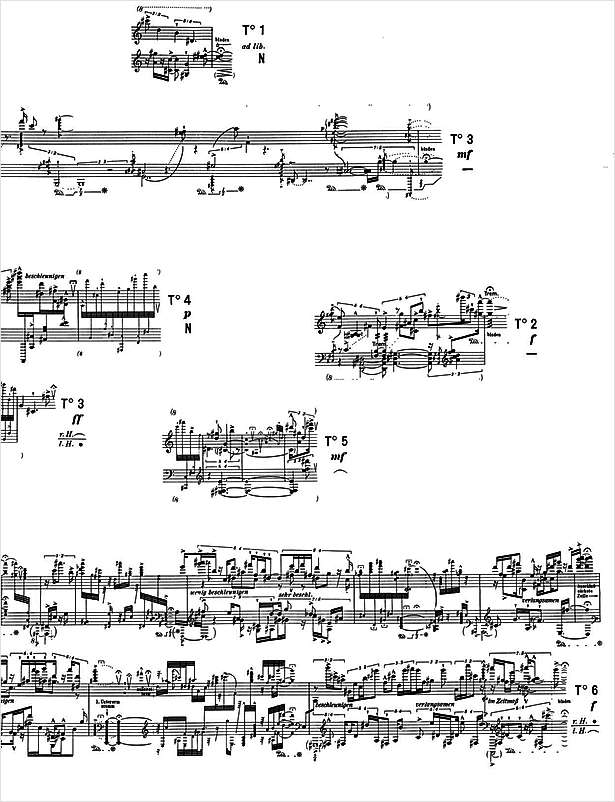
\includegraphics[width=0.9\textwidth]{images/klavierstuck.jpg}
        \end{column}
    \end{columns}~\\
    \vspace{5mm}
    \centering High-level algorithms for the performer
\end{frame}

\subsection{Vocabulary}
\begin{frame}
    \Huge
    \centering{Vocabulary}
\end{frame}    
\begin{frame}[plain]
    \begin{tikzpicture}[remember picture,overlay]
    \node[at=(current page.center)] {
        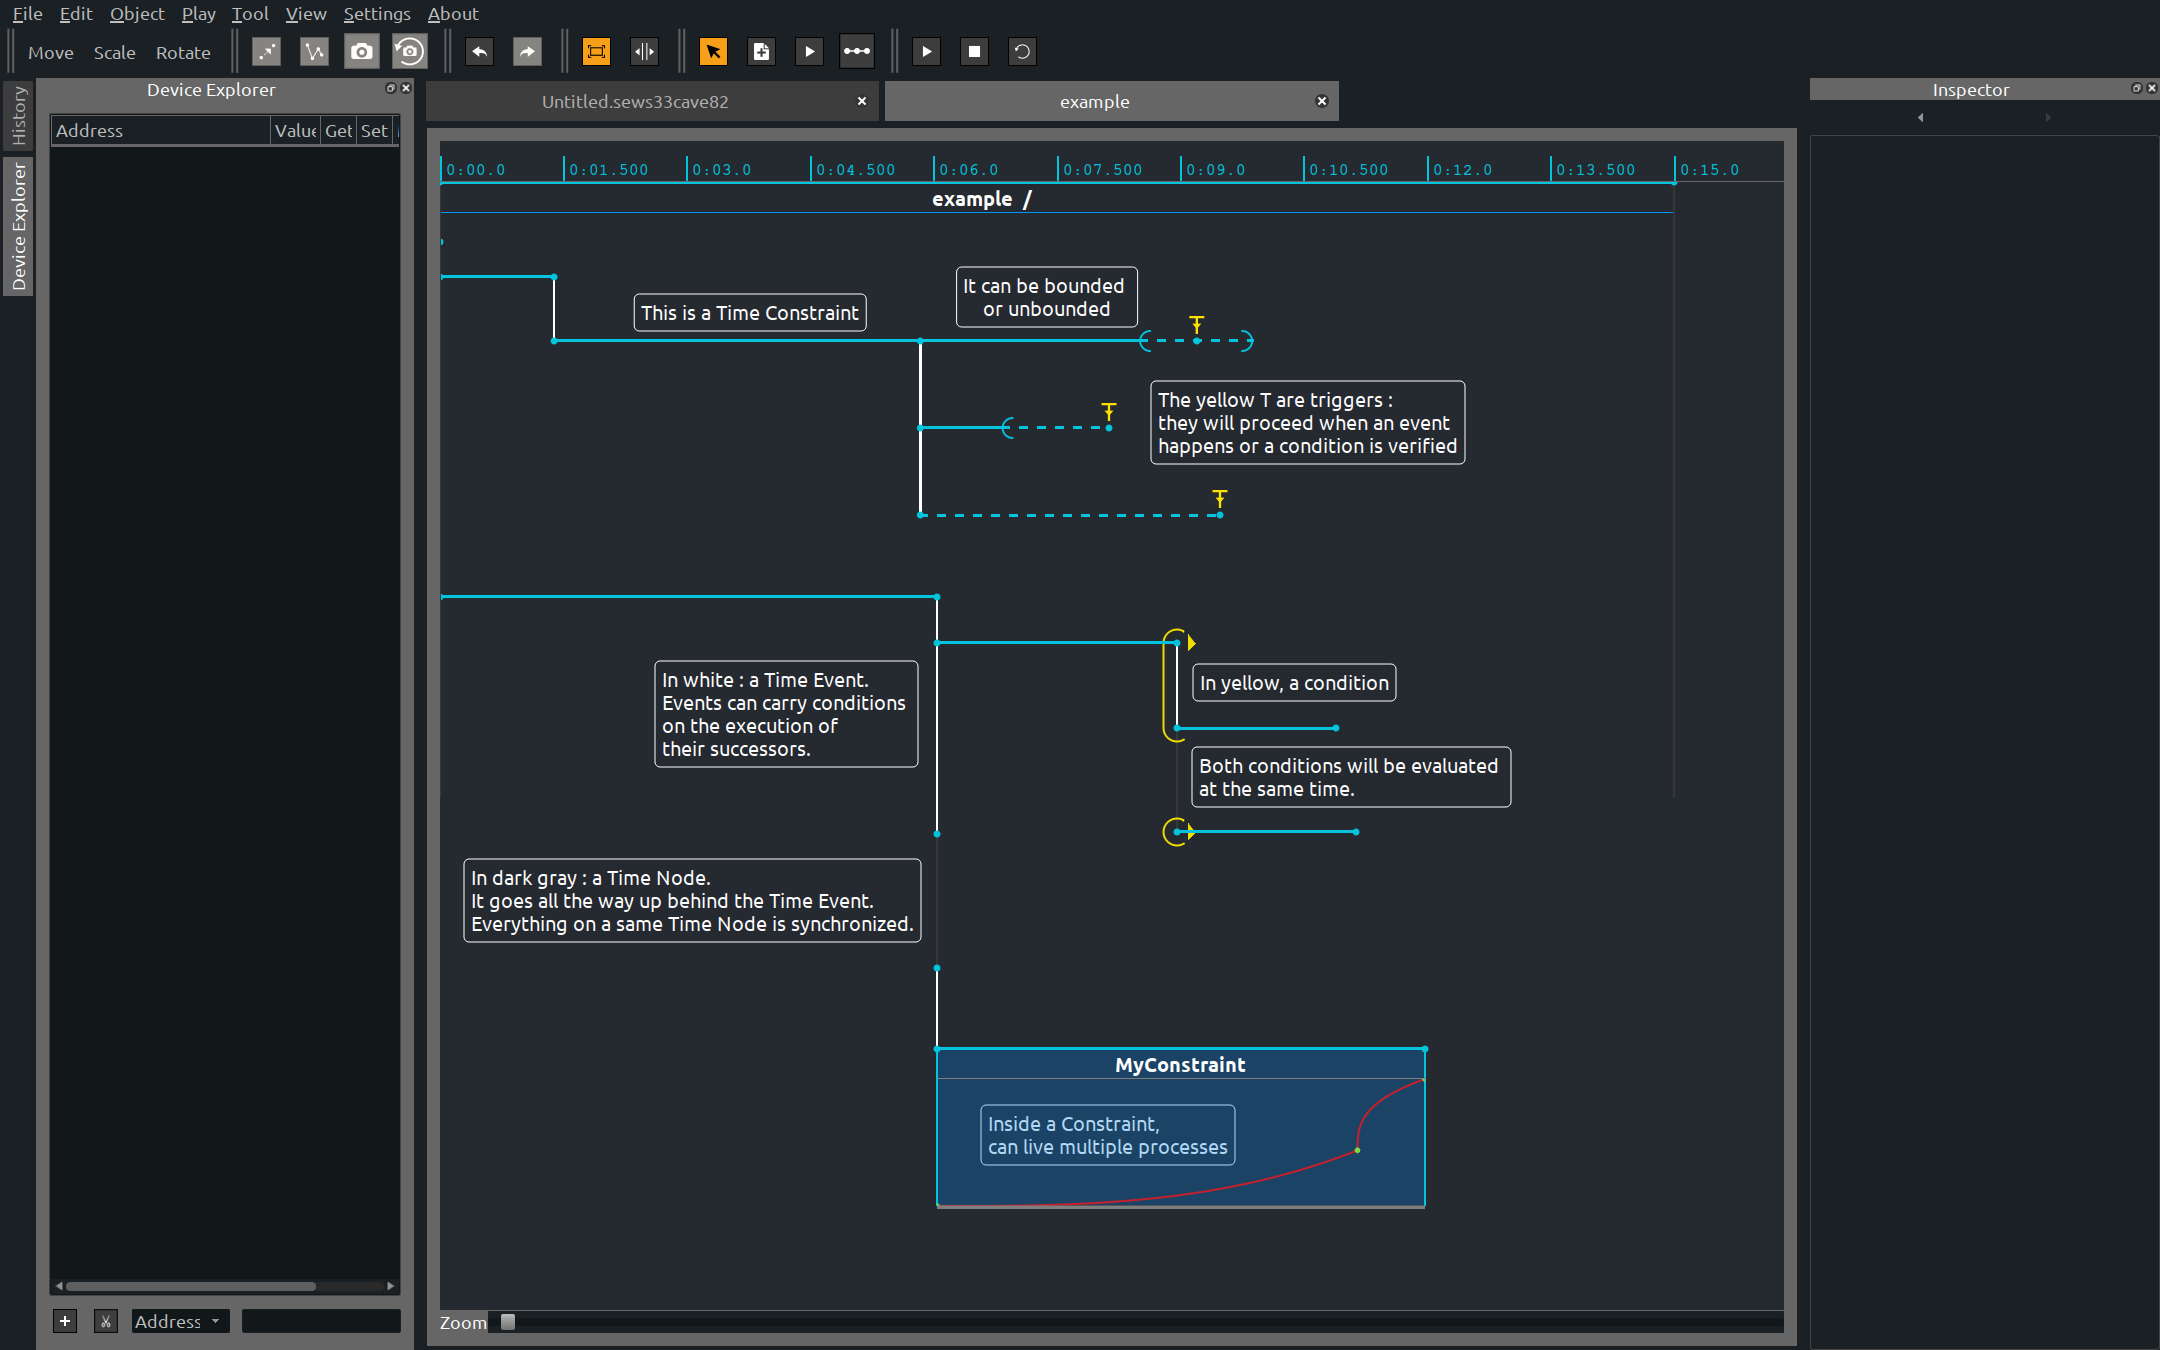
\includegraphics[width=1.5\paperwidth]{images/example.png}
     };
     \end{tikzpicture}
\end{frame}

\section{Authoring}
\subsection{Patterns}
\begin{frame}
    \frametitle{Imperative vs event-driven}
    \begin{figure}
        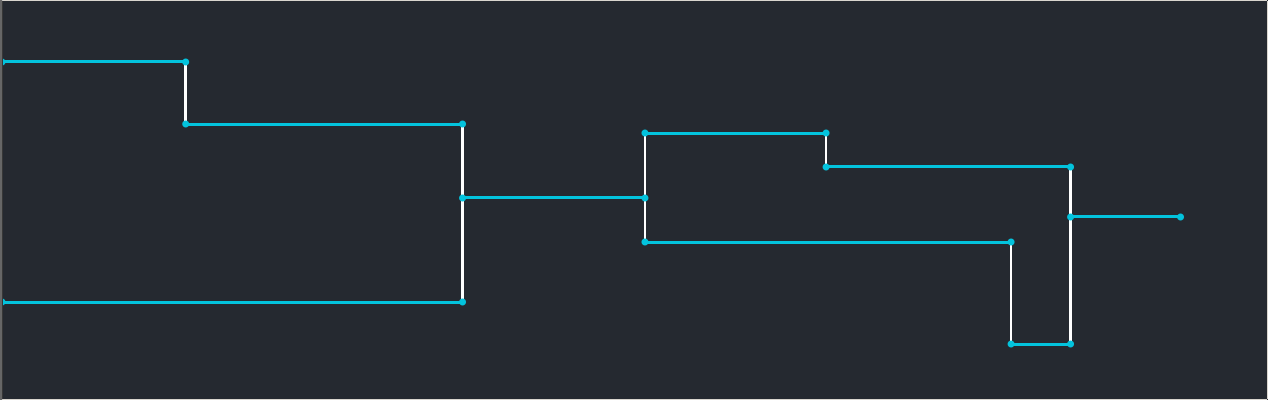
\includegraphics[width=0.7\textwidth]{images/procedural.png}
        \caption{A \emph{then} B}
    \end{figure}~\\
    \begin{figure}
        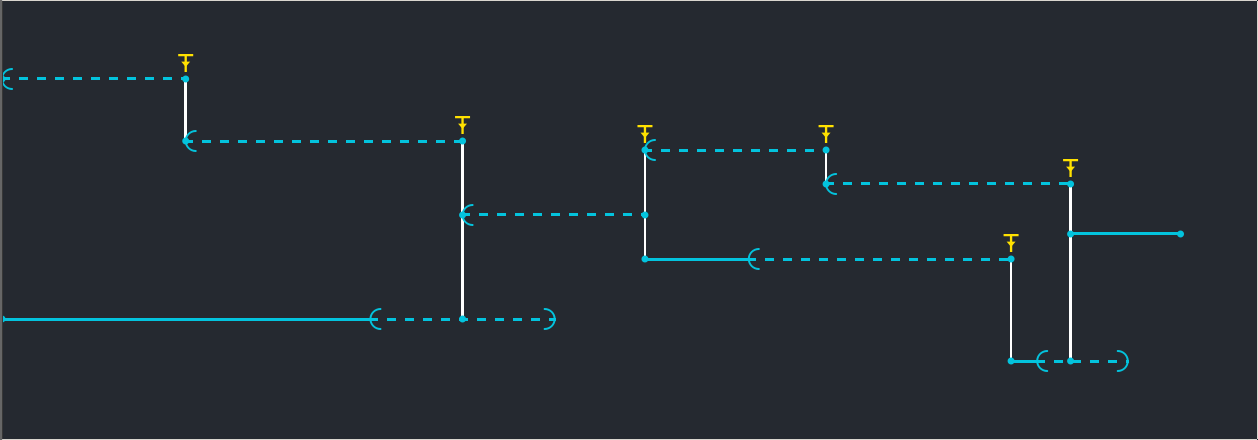
\includegraphics[width=0.7\textwidth]{images/event.png}
        \caption{B \emph{when} A}
    \end{figure}
\end{frame}

\subsection{Loops}
\begin{frame}
    \frametitle{Loops}  
    \Large
    \begin{itemize}
        \item Two interaction points.
        \item One time-constraint.
        \item Allows for \texttt{while} and \texttt{do-while}.
    \end{itemize}
    
    \begin{figure}
        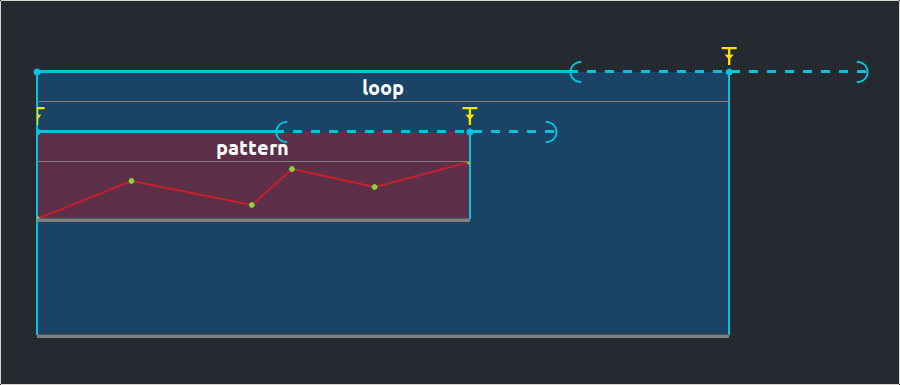
\includegraphics[width=\textwidth]{images/loop.png}
    \end{figure}
\end{frame}

\subsection{Data}
\begin{frame}
    \frametitle{Data tree}  
    \Large
    
    \begin{columns}
        \begin{column}{0.40\textwidth}
            \begin{figure}
                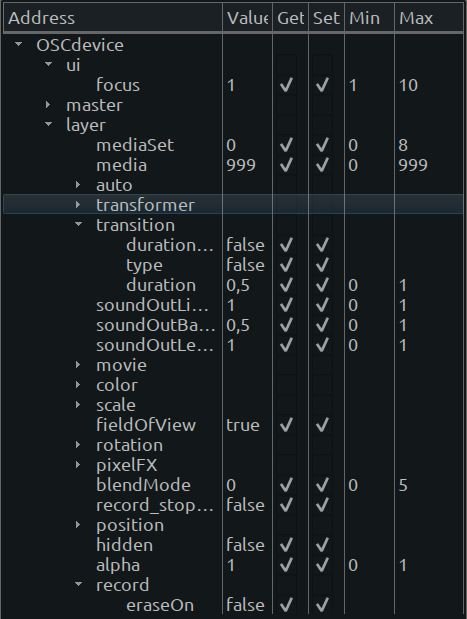
\includegraphics[width=\textwidth]{images/device.png}
            \end{figure}
        \end{column}
        \begin{column}{0.55\textwidth}
            \begin{itemize}
                \item \textbf{Abstraction} over multiple protocols.~\\{\small \textbf{OSC}, \textbf{MIDI}, \textbf{Minuit}, \textbf{HTTP}, \textbf{WebSockets}, \textbf{Serial port}, \textbf{Local intropsection}}...
                \item \textbf{Data model} of (remote) applications.
                \item Can also be used as \textbf{local memory} for the score.
            \end{itemize}
        \end{column}
    \end{columns}
\end{frame}

\subsection{Code}
\begin{frame}
    \frametitle{Code}
    \Large
    i-score: \textbf{temporal language}. 
    \begin{itemize}
    \item Unable to perform arithmetic computations alone. 
    \item Only concerned by \textbf{temporal structure}.
    \item Introduction of an embedded language to perform this work.
    \item Javascript fits the bill.
    \end{itemize}
    
    \Large
\end{frame}

\begin{frame}[fragile]
    \frametitle{Code}
    
    \begin{figure}
        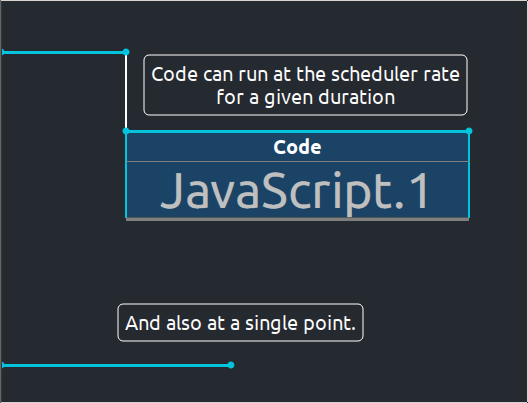
\includegraphics[width=0.45\textwidth]{images/script.png}
    \end{figure}
    
    \begin{lstlisting}
function(t) {       // t in [0; +oo[
var m = new Object; 
m.address = 
    'device:/address'; 
m.value = 
    t + iscore.value('device:/other/address'); 
return [ obj ]; 
}
    \end{lstlisting}
\end{frame}
\begin{frame}[fragile]
    \frametitle{Code}
    
    \begin{figure}
        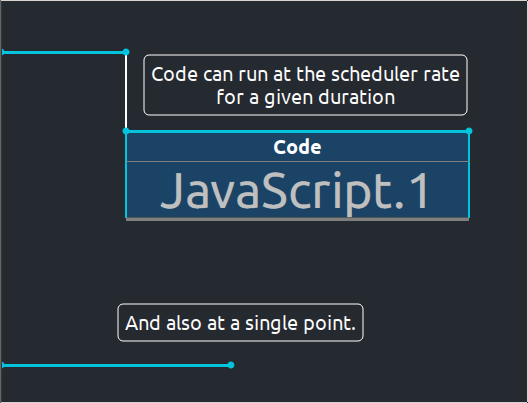
\includegraphics[width=0.45\textwidth]{images/script.png}
    \end{figure}
    
    \begin{lstlisting}
function() {
return [ { 
    address: 'foo:/bar',
    value: Math.Random() * 42 % 35
} ];
\end{lstlisting}
\end{frame}

\begin{frame}
    \frametitle{Procedures}
    Procedures are built from the elements presented up to now.
    
    \begin{figure}
        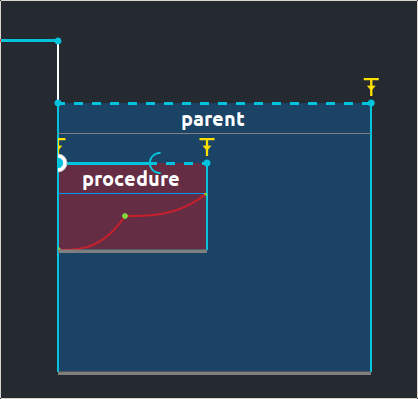
\includegraphics[width=0.45\textwidth]{images/procedure.png}
        \caption{Parent trigger:~\\\texttt{false}~\\First and second sub-triggers:~\\\texttt{local:/p/call == true}}
    \end{figure}
\end{frame}

\section{Demo}

\begin{frame}
    \Huge
    \centering{Demo}~\\\vspace{1cm}
    \url{icmc.blueyeti.fr}
\end{frame}

\section{Conclusion}
\begin{frame}
	\frametitle{Future} 
	\Large
	\begin{itemize}
        \item<1> For the sake of completeness : dynamic allocation primitives.
        \item<2> Hierarchic temporal signatures and work on proper musical features.
        \item<3> Debugging : the main pain point.
        \begin{itemize}
            \item Possibilities that makes sense in the context of artistic creation.
            \item Don't try to force traditional gdb-like debugging.
        \end{itemize}
		
	\end{itemize}
\end{frame}    


\begin{frame}[allowframebreaks]%in case more than 1 slide needed
    
    %remove the icon
    \setbeamertemplate{bibliography item}{}
    
    %remove line breaks
    \setbeamertemplate{bibliography entry title}{}
    \setbeamertemplate{bibliography entry location}{}
    \setbeamertemplate{bibliography entry note}{}
    
    {\footnotesize
        \nocite{*}
        \bibliographystyle{IEEEtran}
        \bibliography{icmc2016}
    }
\end{frame}

\begin{frame}
    \frametitle{Links} 
    \Large
    \begin{itemize}
        \setlength\itemsep{1em}
        \item \textbf{i-score} : \url{www.i-score.org}
    \end{itemize}
        
    \centering
    \vspace{2em}
    \Large{Thanks ! Questions ?}
    \vspace{2em}
    
    \tiny{Uses the Beamer 'simple' theme (Facundo Muñoz); and Mozilla's Fira font family}
\end{frame}
\end{document}
